% ======================================================================================================
% NOTES, TODOS
% ======================================================================================================
% After we select
\section{Study Selection and Refinement}
Finding duplicate that appear in the search result of selected databases is the next phase. Using Zotero tool we merge 40 duplicate papers and we ended up having 175 papers out of the 215 initially retrieved papers. 

The majority of the 175 publications that were chosen are journal articles and conference papers. They contribute correspondingly 60\% and 35\% to the overall outcome. The contribution of articles of the type of book source is, on the otherhand, is low which counts only around 4.5\%. The following pie chart depicts the percentage of articles from 3 main sources, namely, journal, conference paper, and book.  

\begin{figure}[ht]
    \centering
    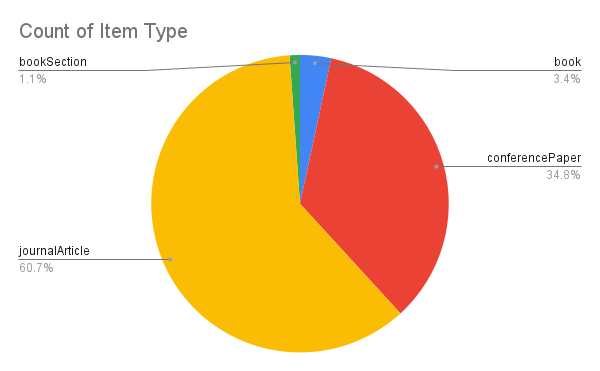
\includegraphics[width=0.6\textwidth]{images/itemtype.png}
    \caption{Percentage of article type based on source type. }
    \label{fig:slr scheme}
\end{figure}

Regarding the publication year, it is noticeable from fig \ref{fig:bar-chart-yaer} that majority of articles published in 2022. The bar-chart also shows that there is an overall increase in security concerns for DT and IoT applications.

\begin{figure}[ht]
    \centering
    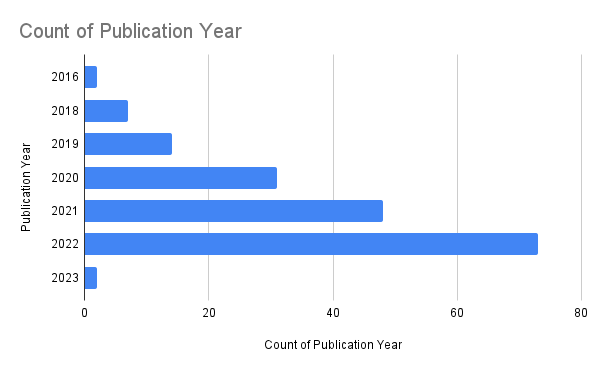
\includegraphics[width=0.8\textwidth]{images/year.png}
    \caption{Number of published papers per year}
    \label{fig:bar-chart-yaer}
\end{figure}


To understand the trend of topic over the 175 paper selected from 2016 to 2023, we analyze the frequency of keywords in the published articles (see Figure \ref{fig:alluvial-key}). Using VOSviewer, we first extract keywords that appear in the article for more than 2 times. Then, we do filtering and sensitization to create a short list of keywords that have more than 6 occurrences. We also merge keywords with similar meaning but different spelling and word variation.  

\begin{figure}[ht]
    \centering
    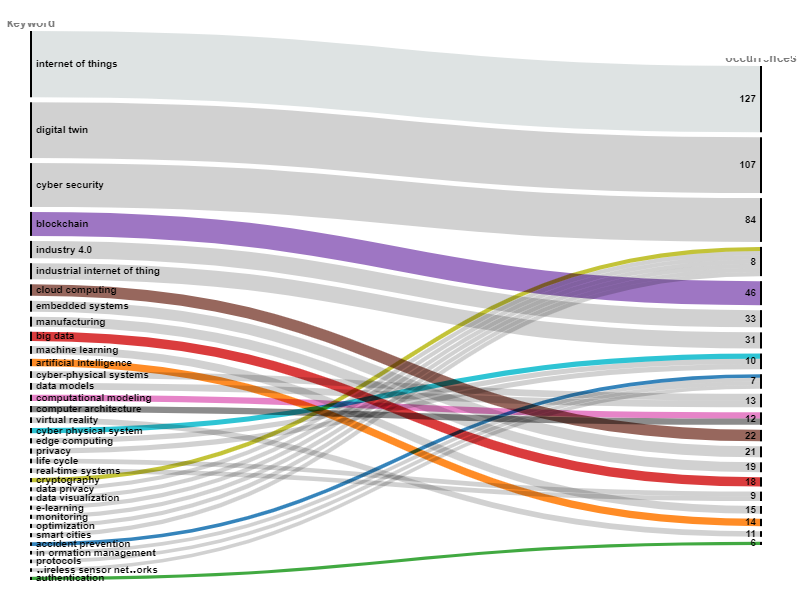
\includegraphics[width=0.95\textwidth]{images/key_belt_png.png}
    % \includesvg[inkscapelatex=false,width=0.95\columnwidth]{images/key_belt.svg}
    \caption{Number of published papers per year}
    \label{fig:alluvial-key}
\end{figure}

The analysis shows that the most frequently mentioned terms in the articles are 'internet of things'(127 occurrences), 'digital twin'(107 occurrences), 'cyber security'(84 occurrences), 'blockchain'(46 occurrences), 'industry 4.0'(33 occurrences), and 'industrial internet of things'(31 occurrences). One noticeable finding from the diagram is the occurrence of the 'authentication' keyword. It only appears six times, which suggests that there is a lack of research on authentication for DT and IoT applications in the literature.  

We also perform keyword co-relationship analysis using VOSviewer to identify cluster of related items. Bibliographic information from 175 papers is used to generate 1187 keywords. Using thesaurus text file, we configure the tool to merge keywords that have similar semantic meaning. Moreover, we set a minimum threshold to limit the result to 87 keywords that meet 3 occurrences of the 1187 keywords.    

\begin{figure}[h]
    % \centering
    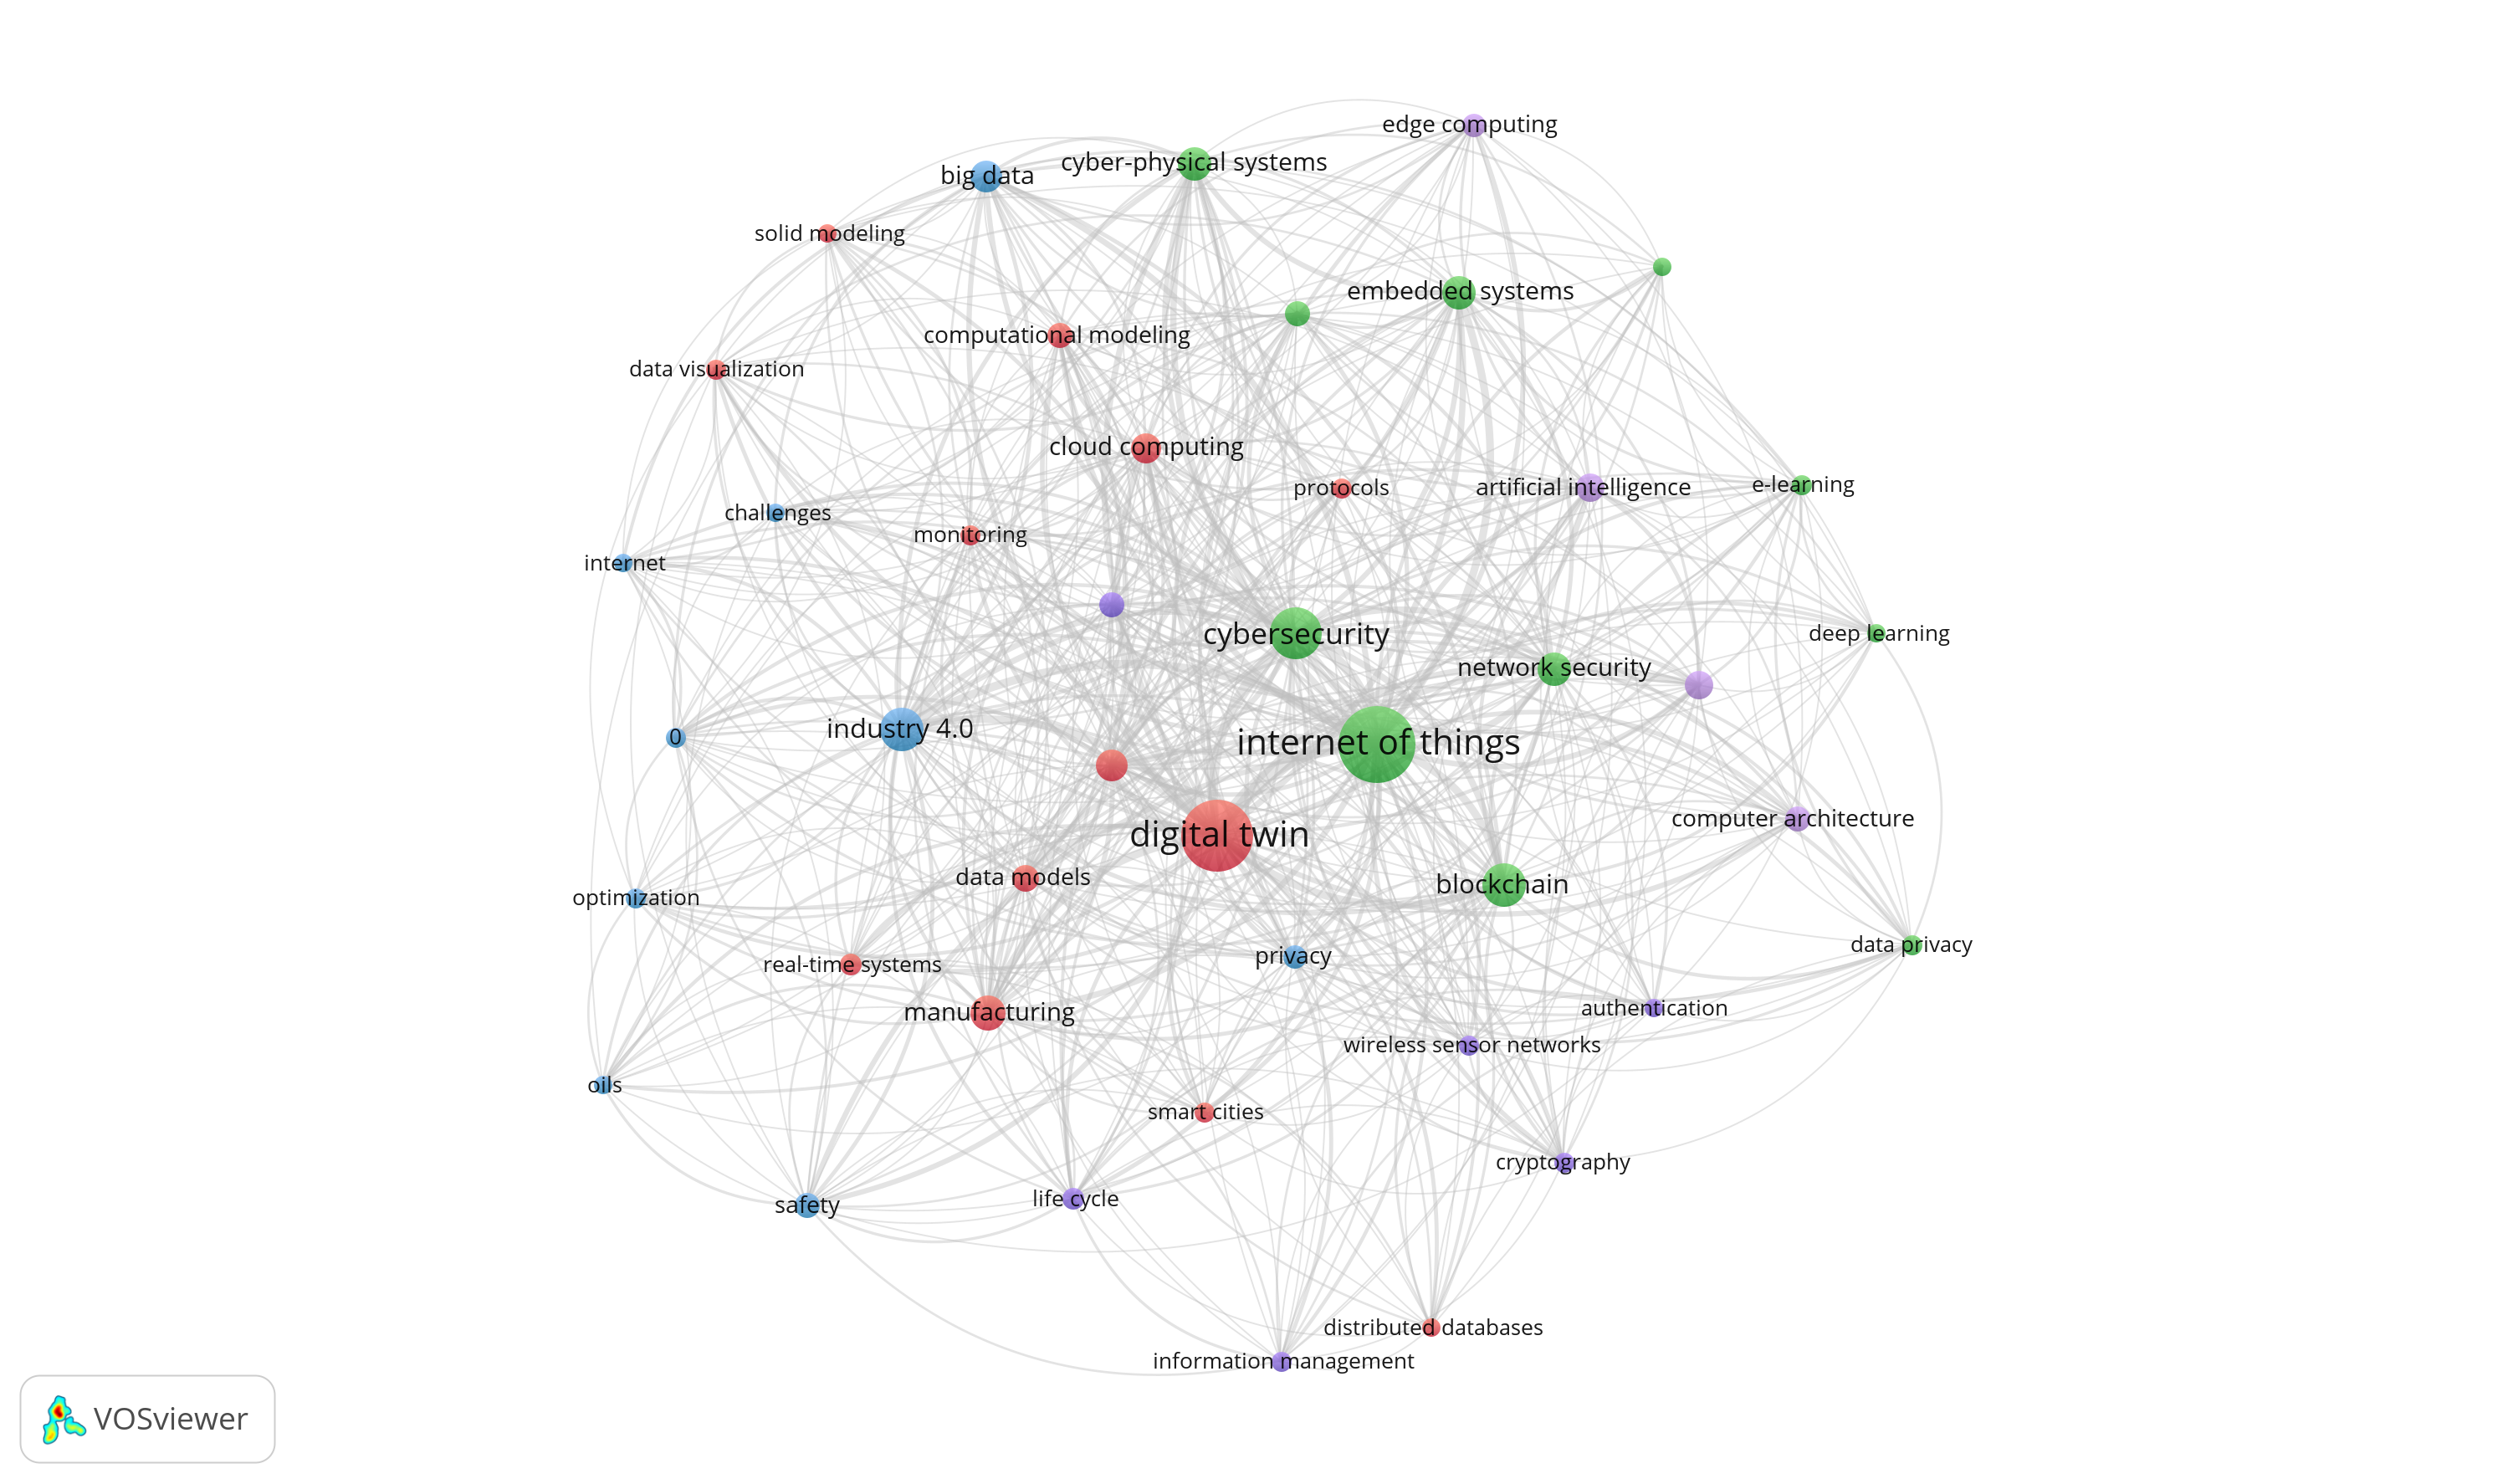
\includegraphics[width=1.5\textwidth, center]{images/vos_key_cooc_6_final.png}
    % \includesvg[inkscapelatex=false,width=0.95\columnwidth]{images/key_belt.svg}
    \caption{keyword co-relationship from VOSviewer}
    \label{fig:co-occurrence-vosv}
\end{figure}

From fig \ref{fig:co-occurrence-vosv} we can identify 5 clusters. Cluster is defined as nodes(terms) that have close relationship - according to the official documentation of VOSviewer. The clusters we identified are: red cluster which includes terms related to digital twin, manufacturing, cloud computing, data models etc. The green cluster which entails keywords related to internet of things, blockchain, network security, cybersecurity, cyber-phsical systems, etc. The thrid cluster are blue. They are related to industry related studies with terms like industry 4.0, optimization, saftey big-data, etc. The fourth cluster has terms that related to machine learning and artifical intelligence. They are represented by purple color.  The last cluster with purple color like the fourth cluster contains few terms related to authentication and cryptography.   